\documentclass[cs4size,a4paper,10pt]{ctexart}   

\linespread{1.5}
\usepackage{geometry}%用于设置上下左右页边距
	\geometry{left=2.5cm,right=2.5cm,top=3.2cm,bottom=2.7cm}
\usepackage{xeCJK,amsmath,paralist,enumerate,booktabs,multirow,graphicx,subfig,setspace,listings,lastpage,hyperref}
\usepackage{amsthm, amssymb, bm, color, framed, graphicx, hyperref, mathrsfs}
\usepackage{mathrsfs}  
	\setlength{\parindent}{2em}
	\lstset{language=Matlab}%
\usepackage{fancyhdr}
\usepackage{graphicx}
\usepackage{subfloat}
\usepackage{listings}
\usepackage{xcolor}
\usepackage{float}
\usepackage{paralist}
\usepackage{setspace}
\usepackage{titlesec}
\usepackage{enumitem}
\usepackage{hyperref}
\usepackage{multirow}
\usepackage{threeparttable}
\usepackage{autobreak}
\usepackage{multicol}
\usepackage{subfig}
\usepackage{unicode-math}
\usepackage{supertabular}

\hypersetup{
	colorlinks=true,
	linkcolor=black,
	urlcolor=black
}

\setenumerate{partopsep=0pt,topsep=0pt}
\setitemize{itemsep=0pt,partopsep=0pt,topsep=0pt}

\titlespacing*{\section}{0pt}{3pt}{3pt}
\titlespacing*{\subsection}{0pt}{2pt}{2pt}
\titlespacing*{\subsubsection}{0pt}{1pt}{1pt}
\titlespacing*{\paragraph}{0pt}{0pt}{0pt}

\ctexset{secnumdepth=4,tocdepth=4}
\setlength{\parindent}{0pt}
\setstretch{1.2}


\setCJKmainfont[BoldFont={FZHei-B01},ItalicFont={FZKai-Z03}]{FZShuSong-Z01} 
\setCJKsansfont[BoldFont={FZHei-B01}]{FZKai-Z03} 
\setCJKmonofont[BoldFont={FZHei-B01}]{FZFangSong-Z02}
\setCJKfamilyfont{zhsong}{FZShuSong-Z01} 
\setCJKfamilyfont{zhhei}{FZHei-B01} 
\setCJKfamilyfont{zhkai}[BoldFont={FZHei-B01}]{FZKai-Z03} 
\setCJKfamilyfont{zhfs}[BoldFont={FZHei-B01}]{FZFangSong-Z02} 
\renewcommand*{\songti}{\CJKfamily{zhsong}} 
\renewcommand*{\heiti}{\CJKfamily{zhhei}} 
\renewcommand*{\kaishu}{\CJKfamily{zhkai}} 
\renewcommand*{\fangsong}{\CJKfamily{zhfs}}


\definecolor{mKeyword}{RGB}{0,0,255}          % bule
\definecolor{mString}{RGB}{160,32,240}        % purple
\definecolor{mComment}{RGB}{34,139,34}        % green
\definecolor{mNumber}{RGB}{128,128,128} 

\lstdefinestyle {njulisting} {
	basewidth = 0.5 em,
	lineskip = 3 pt,
	basicstyle = \small\ttfamily,
	% keywordstyle = \bfseries,
	commentstyle = \itshape\color{gray}, 
	basicstyle=\small\ttfamily,
	keywordstyle={\color{black}},     % sets color for keywords
	stringstyle={\color{black}},       % sets color for strings
	commentstyle={\color{black}},     % sets color for comments
	numberstyle=\tiny\color{black},
	numbers = left,
	captionpos = t,
	breaklines = true,
	xleftmargin = 1 em,
	xrightmargin = 0 em,
	frame=tlrb,
	tabsize=4,
	aboveskip = 7 pt, %与代码环境上一行的垂直间距
    belowskip = -2 pt %与代码环境下一行的垂直间距
}

\lstset{
style = njulisting, % 调用上述样式 
flexiblecolumns % 允许调整字符宽度
}

\newcommand \sverb {\ \verb}

%================= 基本格式预置 ===========================
\usepackage{fancyhdr}
\pagestyle{fancy}
\lhead{数据管理基础}
\rhead{关系数据库标准语言SQL}
\cfoot{\thepage}
\renewcommand{\headrulewidth}{0.4pt}
\renewcommand{\theenumi}{(\arabic{enumi})}
\CTEXsetup[format={\bfseries\zihao{-3}}]{section}
\CTEXsetup[format={\bfseries\zihao{4}}]{subsection}
\CTEXsetup[format={\bfseries\zihao{-4}}]{subsubsection}


\renewcommand{\contentsname}{目录}  
\begin{document}

	\begin{center}
		{\huge\textbf{第三章\ 关系数据库标准语言SQL}}
	\end{center}
	%---------目录---------% 
	\pagenumbering{Roman}
	\tableofcontents
	\clearpage

 	%---------正文---------% 
	\pagenumbering{arabic}
	\setcounter{page}{1}
	\setlength{\parskip}{0.65em}

	\setlength\abovedisplayskip{5pt}
	\setlength\belowdisplayskip{5pt}

	\section{SQL概述}
\begin{itemize}
    \item 结构化查询语言(Structured Query Language,SQL),是关系数据库的标准语言,也是一个通用的、功能极强的关系数据库语言
    \item 目前没有一个数据库系统能够支持 SQL 标准的所有概念和特性
    \item 许多软件厂商对 SQL 基本命令集还进行了不同程度的扩充和修改,又可以支持标准以外的一些功能特性
    \item SQL 的特点
    \begin{itemize}
        \item 综合统一
        \item 高度非过程化
        \item 面向集合的操作方式
        \item 以同一种语法结构提供多种使用方式
        \item 语言简洁,易学易用
    \end{itemize}
    \item 支持 SQL 的关系数据库管理系统同样支持关系数据库三级模式结构,其中外模式包含若干\textbf{视图}和部分\textbf{基本表},模式包括若干基本表,内模式包含若干\textbf{存储文件}
    \begin{itemize}
        \item 基本表
        \begin{itemize}
            \item 本身独立存在的表
            \item SQL 中一个关系就对应一个基本表
            \item 一个(或多个)基本表对应一个存储文件
            \item 一个表可以带若干索引
        \end{itemize}
        \item 存储文件
        \begin{itemize}
            \item 逻辑结构组成了关系数据库的内模式
            \item 物理结构对用户是隐蔽的
        \end{itemize}
        \item 视图
        \begin{itemize}
            \item 从一个或几个基本表导出的表
            \item 数据库中只存放视图的定义而不存放视图对应的数据
            \item 视图是一个虚表
            \item 用户可以在视图上再定义视图
        \end{itemize}
    \end{itemize}
\end{itemize}

\begin{figure}[H]
    \vspace{-0.5em}
	\centering
	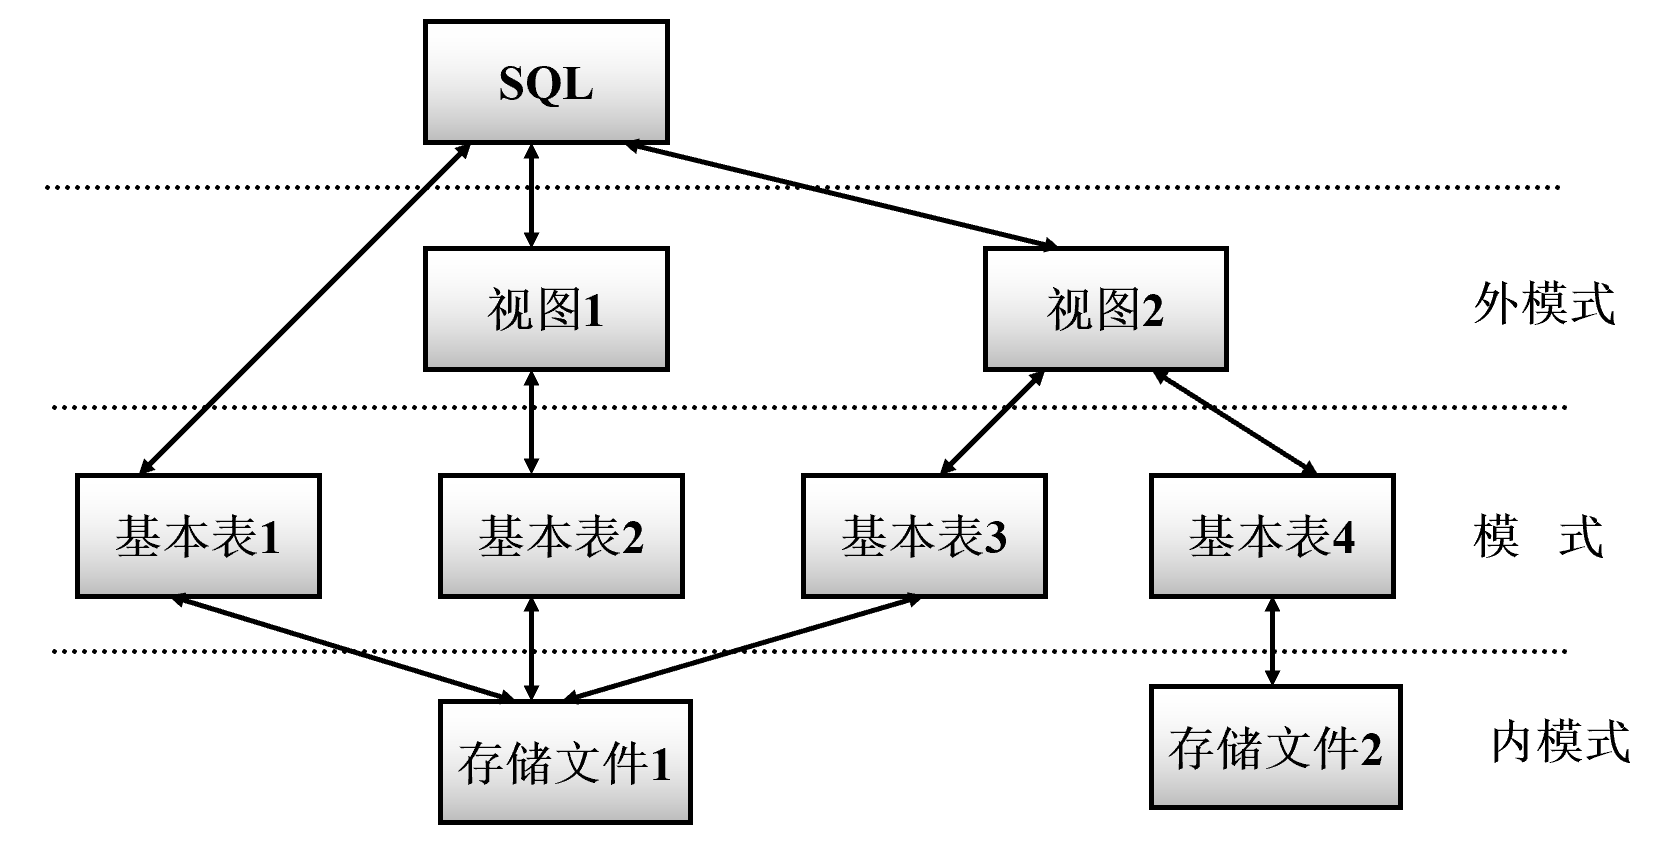
\includegraphics[width=0.55\textwidth]{images/3.1}
    \vspace{-1em}
\end{figure}

\section{数据定义}
\begin{itemize}
    \item 层次化的数据库对象命名机制
    \begin{itemize}
        \item 一个关系数据库管理系统的实例中可以建立多个数据库
        \item 一个数据库中可以建立多个模式
        \item 一个模式下通常包括多个表、视图和索引等数据库对象
    \end{itemize}
    \begin{figure}[H]
        \vspace{-0.5em}
        \centering
        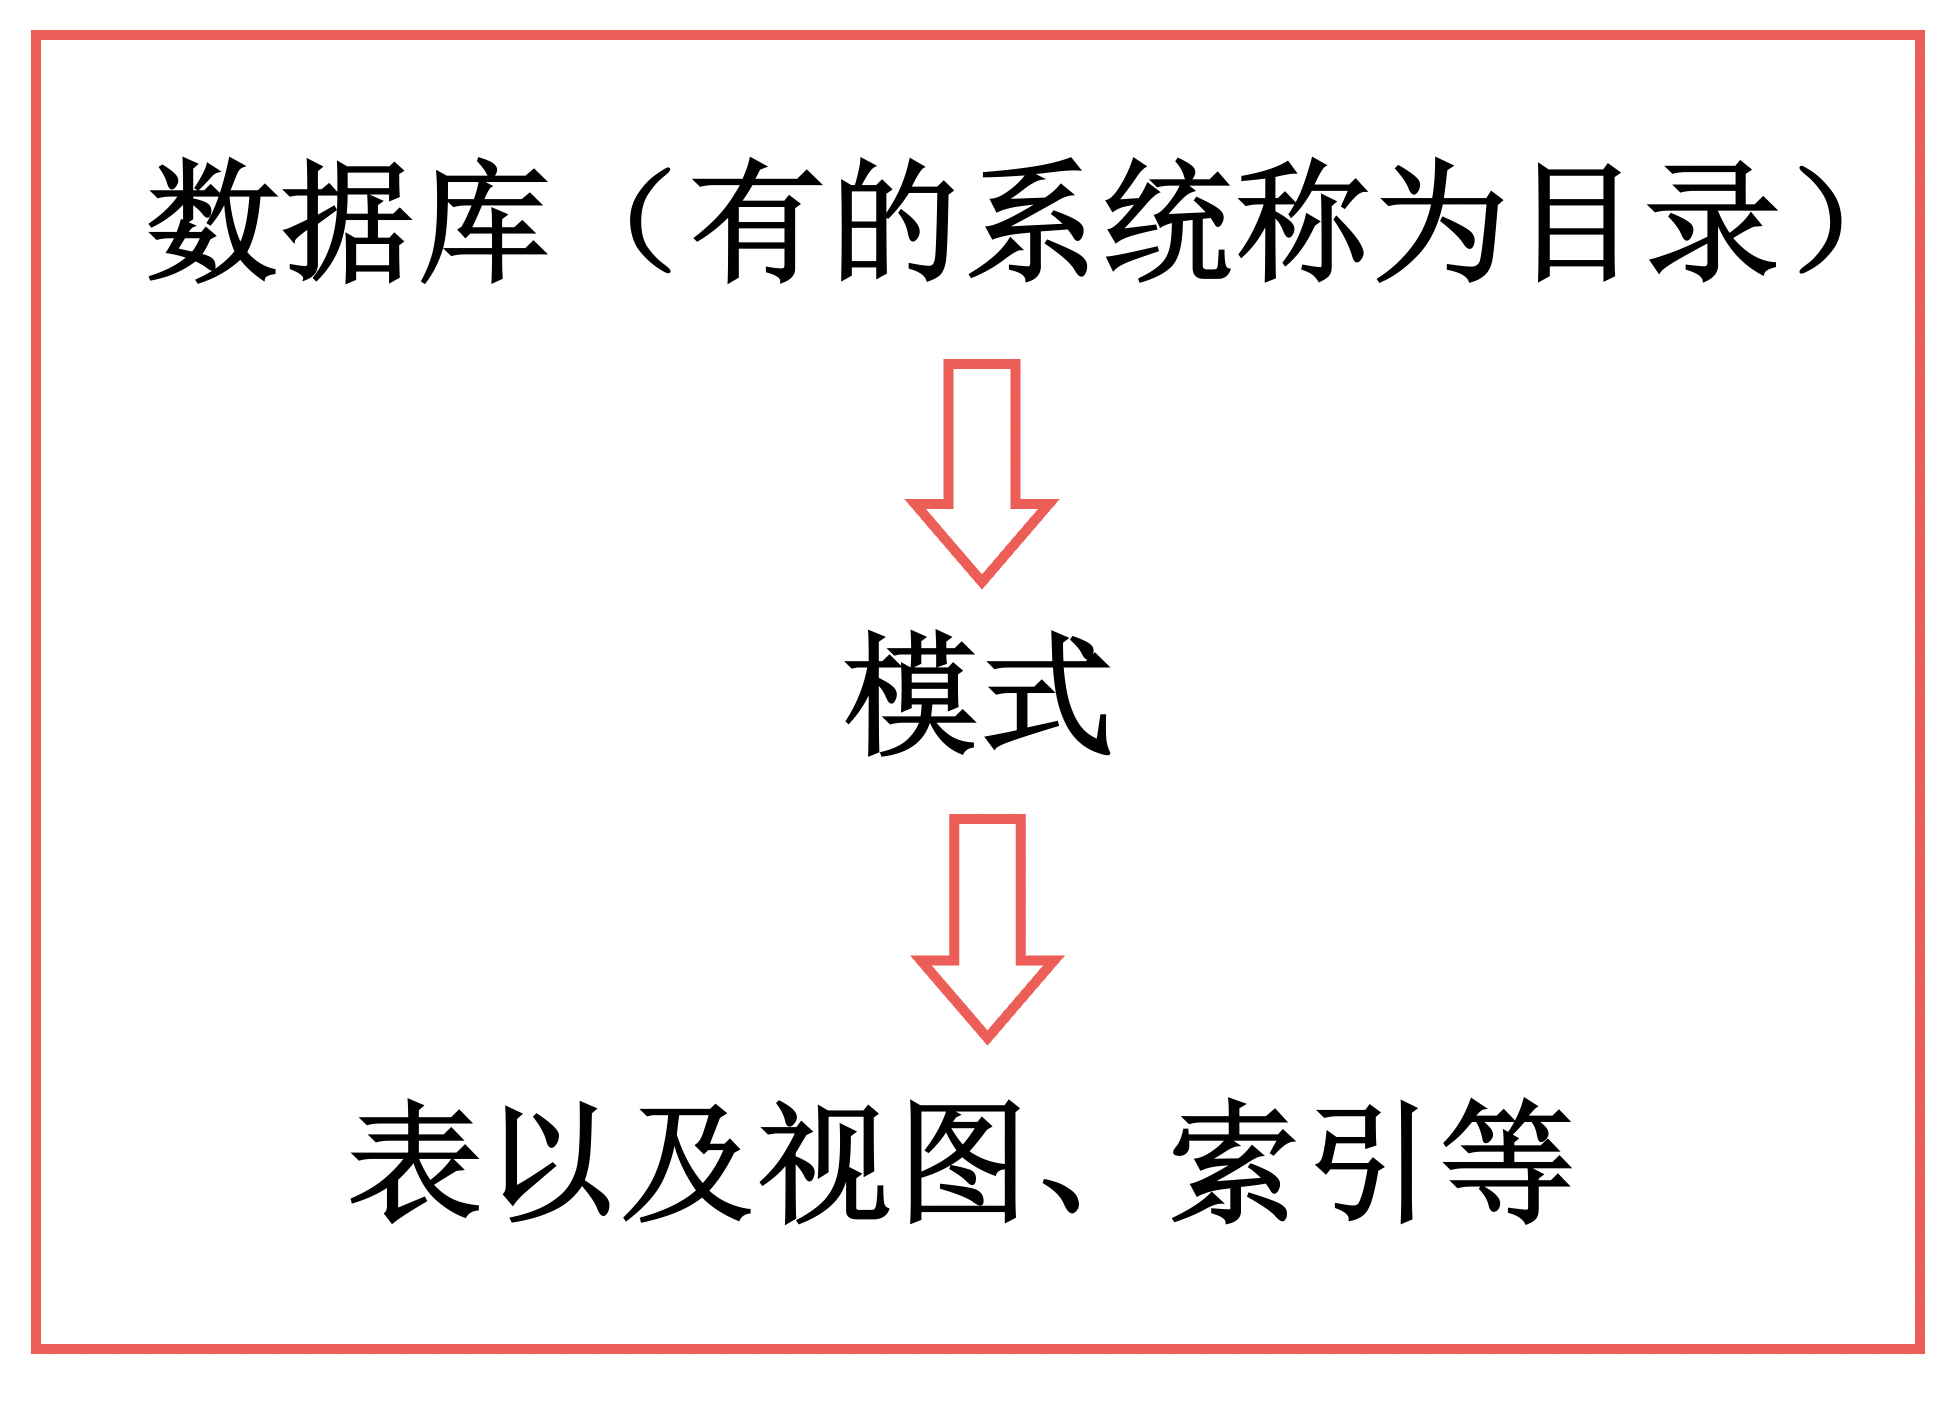
\includegraphics[width=0.3\textwidth]{images/3.2}
        \vspace{-1em}
    \end{figure}
    \item SQL的数据定义功能
\end{itemize}

\begin{table}[H]
    \vspace{-0.5em}
    \centering
    \begin{tabular}{|c|c|c|c|}
    \hline
    \textbf{操作对象} & \textbf{创建}   & \textbf{删除} & \textbf{修改} \\ \hline
    模式            & \verb|CREATE SCHEMA| & \verb|DROP SCHEMA| &             \\ \hline
    表             & \verb|CREATE TABLE|  & \verb|DROP TABLE|  & \verb|ALTER TABLE| \\ \hline
    视图            & \verb|CREATE VIEW|  & \verb|DROP VIEW|  &             \\ \hline
    索引            & \verb|CREATE INDEX|  & \verb|DROP INDEX|  & \verb|ALTER INDEX|\\ \hline
    \end{tabular}
    \vspace{-1em}
\end{table}

\subsection{模式的定义与删除}

\subsubsection{定义模式}
定义模式实际上定义了一个命名空间。在这个空间中可以定义该模式包含的数据库对象,例如基本表、视图、索引等

SQL 中模式定义语句为
\begin{lstlisting}[language=sql]
CREATE SCHEMA <模式名> AUTHORIZATION <用户名>;
\end{lstlisting}
\begin{itemize}
    \item 在\sverb|CREATE SCHEMA|\ 中可以接受\sverb|CREATE TABLE|,\sverb|CREATE VIEW| 和 \sverb|GRANT|\ 子句,即
\end{itemize}
\begin{lstlisting}[language=sql]
CREATE SCHEMA <模式名> AUTHORIZATION <用户名> [<表定义子句> | <视图定义子句> | <授权定义子句>]
\end{lstlisting}

\subsubsection{删除模式}
SQL 中删除模式的语句为
\begin{lstlisting}[language=sql]
DROP SCHEMA <模式名> <CASCADE|RESTRICT>;
\end{lstlisting}

\begin{itemize}
    \item 其中\sverb|CASCADE|和\sverb|RESTRICT|\ 两者必选其一
    \begin{itemize}
        \item 选择了 \sverb|CASCADE|(级联),表示在删除模式的同时把该模式中所有的数据库对象全部删除
        \item 选择了\sverb|RESTRICT| (限制),表示如果该模式中定义了下属的数据库对象(如表、视图等),则拒绝该删除语句的执行。仅当该模式中没有任何下属的对象时才能执行\sverb|DROP SCHEMA|\ 语句
    \end{itemize}
\end{itemize}

\subsection{基本表的定义、删除与修改}

\subsubsection{定义基本表}
SQL 中定义基本表的格式为
\begin{lstlisting}[language=sql]
CREATE TABLE <表名>
    (<列名> <数据类型> [<列级完整性约束条件>]
    [,<列名> <数据类型>[<列级完整性约束条件>]] 
   	…
    [,<表级完整性约束条件>]);
\end{lstlisting}

\begin{itemize}
    \item \verb|<表名>|:所要定义的基本表的名字
    \item \verb|<列名>|:组成该表的各个属性(列)
    \item \verb|<列级完整性约束条件>|:涉及相应属性列的完整性约束条件
    \item \verb|<表级完整性约束条件>|:涉及一个或多个属性列的完整性约束条件 
    \item 如果完整性约束条件涉及到该表的多个属性列,则必须定义在表级上,否则既可以定义在列级也可以定义在表级
\end{itemize}

\subsubsection{数据类型}
\begin{itemize}
    \item SQL 中域的概念用数据类型来实现
    \item 定义表的属性时需要指明其数据类型及长度 
    \item 一个属性选用哪种数据类型一般从取值范围和要做哪些运算两方面来考虑
\end{itemize}

\subsubsection{修改基本表}
SQL 中修改基本表的格式为
\begin{lstlisting}[language=sql]
ALTER TABLE <表名>
[ADD[COLUMN] <新列名> <数据类型> [完整性约束]]
[ADD <表级完整性约束>]
[DROP [COLUMN] <列名> [CASCADE | RESTRICT]]
[DROP CONSTRAINT <完整性约束名> [RESTRICT | CASCADE]]
[ALTER COLUMN <列名> <数据类型>];
\end{lstlisting}

\begin{itemize}
    \item \verb|<表名>|\ 是要修改的基本表
    \item \verb|ADD|\ 子句用于增加新列、新的列级完整性约束条件和新的表级完整性约束条件
    \item \verb|DROP COLUMN|\ 子句用于删除表中的列
    \begin{itemize}
        \item 如果指定了\sverb|CASCADE|\ 短语,则自动删除引用了该列的其他对象
        \item 如果指定了\sverb|RESTRICT|\ 短语,则如果该列被其他对象引用,关系数据库管理系统将拒绝删除该列
    \end{itemize}
    \item  \verb|DROP CONSTRAINT|\ 子句用于删除指定的完整性约束条件
    \item  \verb|ALTER COLUMN|\ 子句用于修改原有的列定义,包括修改列名和数据类型
\end{itemize}

\subsubsection{删除基本表}
SQL 删除基本表的格式为
\begin{lstlisting}[language=sql]
DROP TABLE <表名> [RESTRICT| CASCADE];
\end{lstlisting}
\begin{itemize}
    \item 若选择\sverb|RESTRICT|,则删除表是有限制的:欲删除的基本表不能被其他表的约束所引用,如果存在依赖该表的对象,则此表不能被删除
    \item 若选择\sverb|CASCADE|,删除该表没有限制:在删除基本表的同时,相关的依赖对象一起删除 
\end{itemize}

\subsection{索引的建立和删除}
\begin{itemize}
    \item 建立索引的目的:加快查询速度
    \begin{itemize}
        \item 由数据库管理员或表的拥有者建立
        \item 由关系数据库管理系统自动完成维护
        \item 关系数据库管理系统自动使用合适的索引作为存取路径,用户不必也不能显式地选择索引
    \end{itemize}
    \item 关系数据库管理系统中常见索引:
    \vspace{-1em}
	\begin{multicols}{2}
        \begin{itemize}
            \item 顺序文件上的索引
            \item B+树索引
            \item 散列索引
            \item 位图索引
        \end{itemize}
	\end{multicols}
	\vspace{-1em}
\end{itemize}

\subsubsection{建立索引}
建立索引的语句格式为
\begin{lstlisting}[language=sql]
CREATE [UNIQUE] [CLUSTER] INDEX <索引名> 
ON <表名> (<列名> [<次序>] [,<列名> [<次序>]]…);
\end{lstlisting}

\begin{itemize}
    \item \verb|<表名>|:要建索引的基本表的名字
    \item \verb|索引|:可以建立在该表的一列或多列上,各列名之间用逗号分隔
    \item \verb|<次序>|:指定索引值的排列次序,升序为\sverb|ASC|,降序为\sverb|DESC|,缺省值为 \sverb|ASC|
    \item \verb|UNIQUE|:此索引的每一个索引值只对应唯一的数据记录
    \item \verb|CLUSTER|:表示要建立的索引是聚簇索引
\end{itemize}

\subsubsection{修改索引}
对于已建立的索引,如果需要对其重新命名,语句格式为
\begin{lstlisting}[language=sql]
ALTER INDEX <旧索引名> RENAME TO <新索引名>
\end{lstlisting}

\subsubsection{删除索引}
删除索引的语句格式为
\begin{lstlisting}[language=sql]
DROP INDEX <索引名>;
\end{lstlisting}

\subsection{数据字典}
数据字典是关系数据库管理系统内部的一组系统表,它记录了数据库中所有定义信息:
\vspace{-0.8em}
\begin{multicols}{2}
    \begin{itemize}
        \item 关系模式定义
        \item 视图定义
        \item 索引定义
        \item 完整性约束定义
        \item 各类用户对数据库的操作权限
        \item 统计信息等
    \end{itemize}
\end{multicols}
\vspace{-1em}

关系数据库管理系统在执行 SQL 的数据定义语句时,实际上就是在更新数据字典表中的相应信息

\section{数据查询}
SQL 提供了\sverb|SELETE|\ 语句进行数据查询,该语句具有灵活的使用方式和丰富的功能,其一般格式为
\begin{lstlisting}[language=sql]
SELECT [ALL|DISTINCT] <目标列表达式> [,<目标列表达式>] …
FROM <表名或视图名> [,<表名或视图名>…] | (SELECT语句) [AS] <别名>
[WHERE <条件表达式>]
[GROUP BY <列名1> [HAVING <条件表达式>]]
[ORDER BY <列名2> [ASC | DESC]];
\end{lstlisting}
\begin{itemize}
    \item \verb|SELECT|\ 子句:指定要显示的属性列
    \item \verb|FROM|\ 子句:指定查询对象(基本表或视图)
    \item \verb|WHERE|\ 子句:指定查询条件
    \item \verb|GROUP BY|\ 子句:对查询结果按指定列的值分组,该属性列值相等的元组为一个组。通常会在每组中作用聚集函数。
    \item \verb|HAVING|\ 短语:只有满足指定条件的组才予以输出
    \item \verb|ORDER BY|\ 子句:对查询结果表按指定列值的升序或降序排序 
\end{itemize}

以下例子均来源于下图的学生-课程数据库
\begin{figure}[H]
    \vspace{-0.5em}
    \centering
    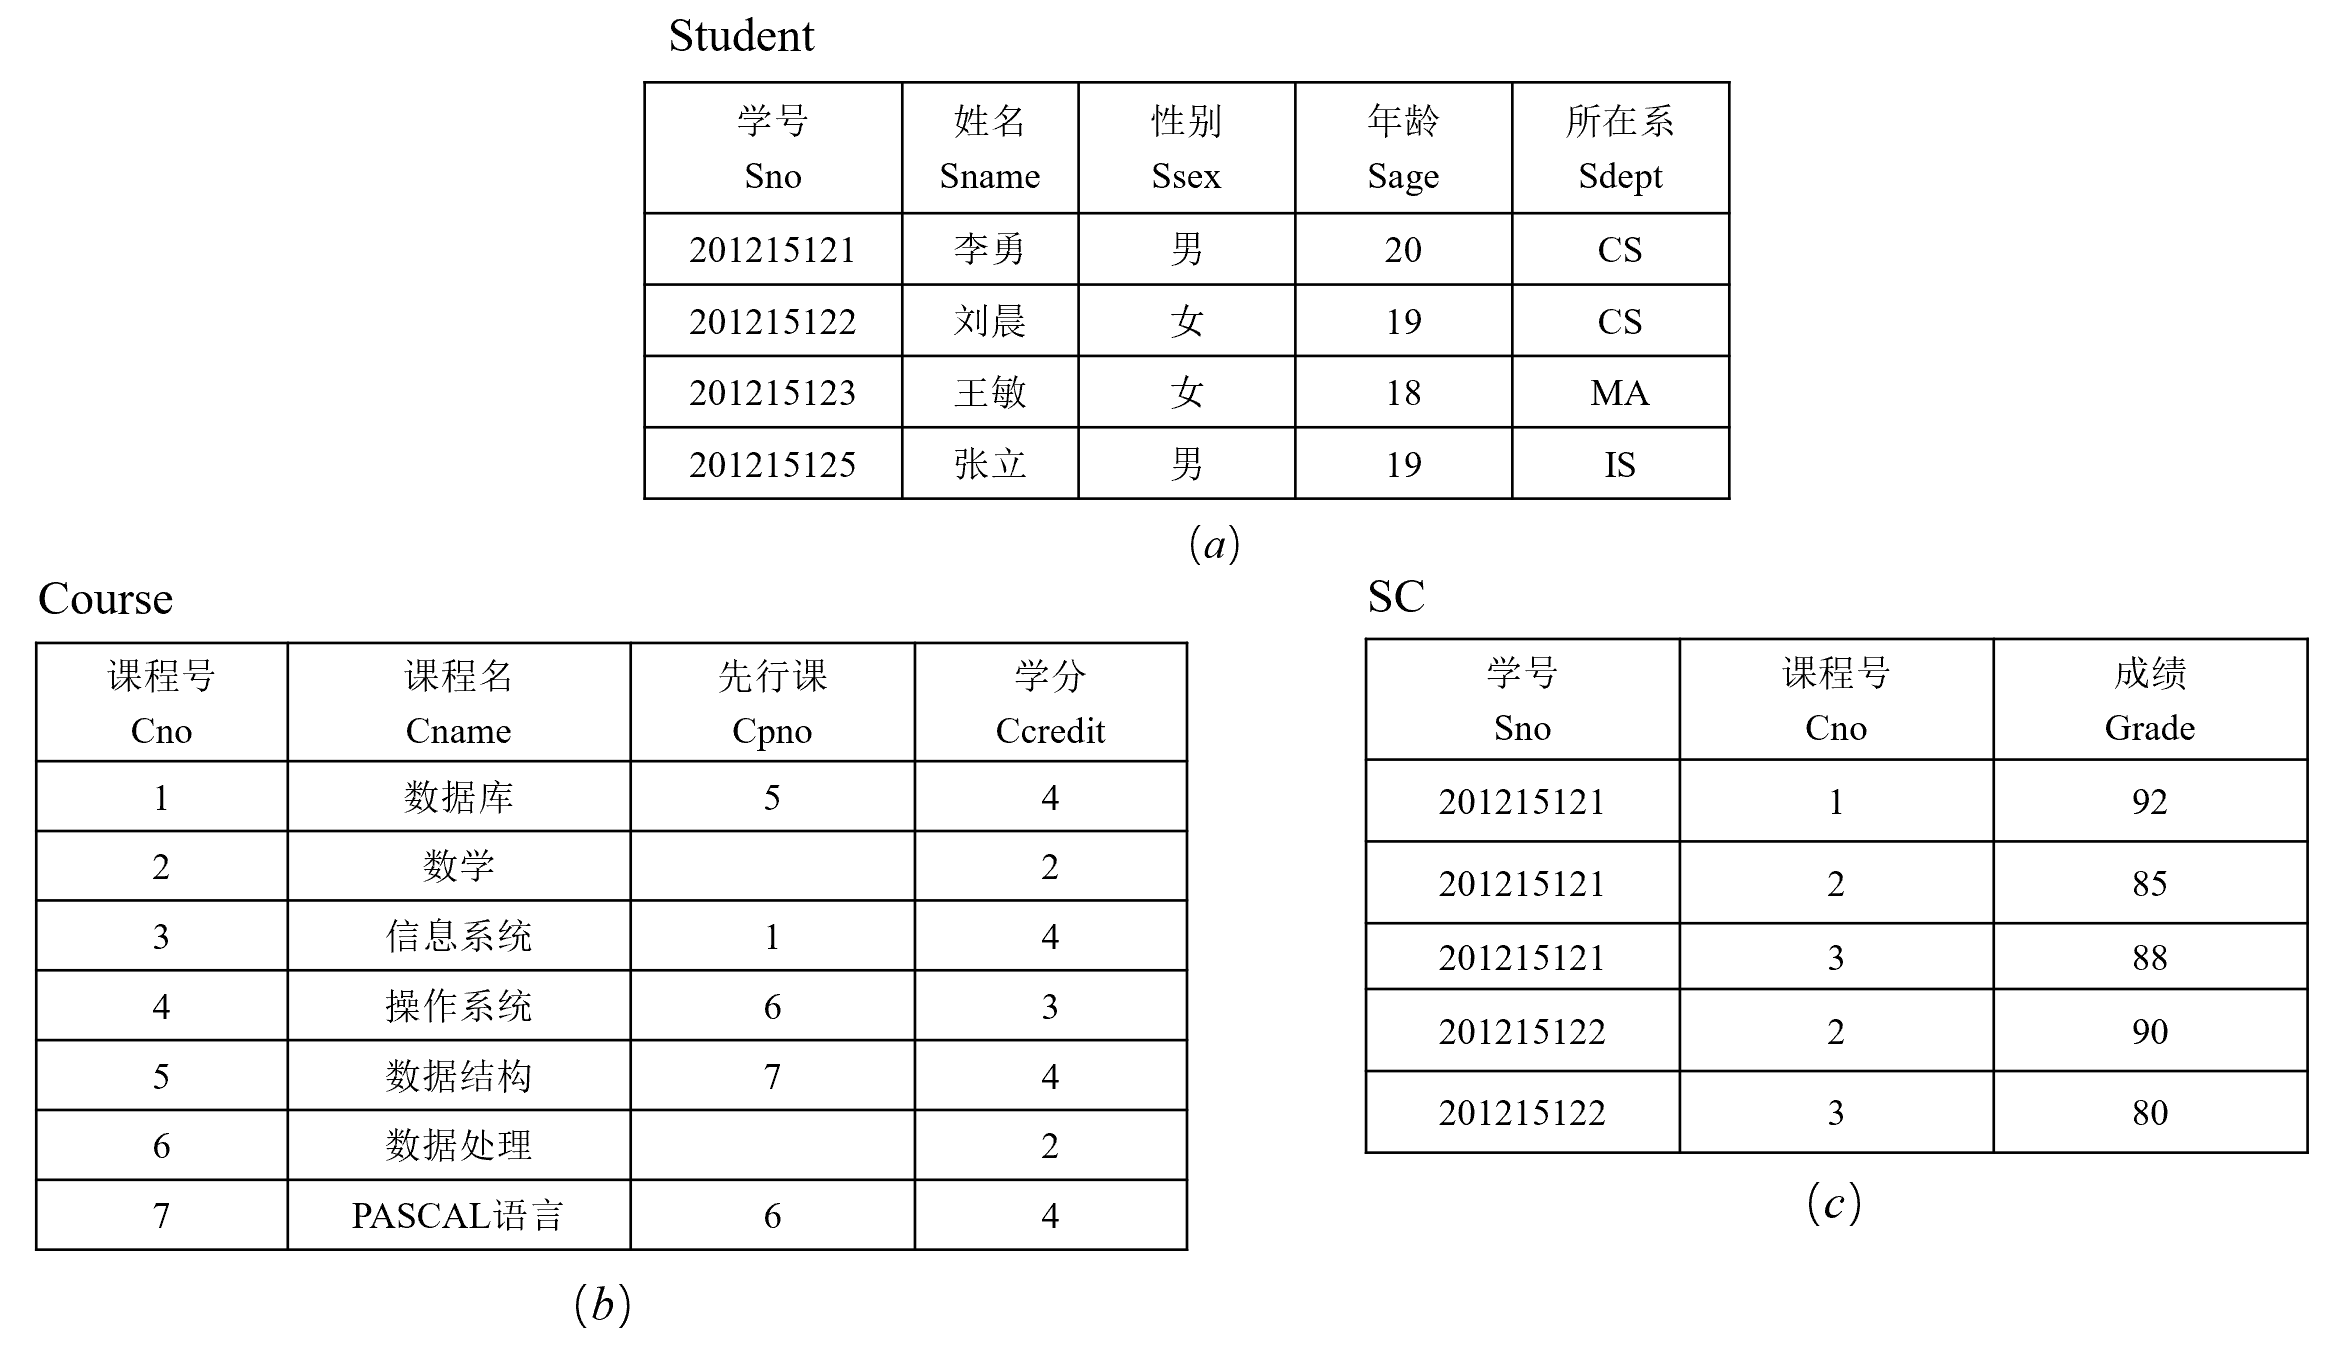
\includegraphics[width=0.85\textwidth]{images/2.3.2}
    \vspace{-1em}
\end{figure}

\subsection{单表查询}

\subsubsection{选择表中的若干列}
查询指定列:查询全体学生的学号与姓名
\begin{lstlisting}[language=sql]
SELECT DISTINCT Sno
FROM SC; 
\end{lstlisting}

查询全部列:查询全体学生的详细记录
\begin{lstlisting}[language=sql]
SELECT  *
FROM Student;
\end{lstlisting}

查询经过计算的值:查询全体学生的姓名、出生年份和所在的院系,要求用小写字母表示系名,且使用列别名改变查询结果的列标题
\begin{lstlisting}[language=sql]
SELECT Sname NAME, 'Year of Birth:' BIRTH, 2014-Sage BIRTHDAY, LOWER(Sdept) DEPARTMENT
FROM Student;
\end{lstlisting}

查询结果为:(当前年为2014年)
\begin{table}[H]
    \vspace{-0.5em}
    \centering
    \resizebox{0.56\textwidth}{!}{
        \begin{tabular}{|c|c|c|c|}
        \hline
        NAME & BIRTH          & BIRTHDAY & DEPARTMENT \\ \hline
        李勇   & Year of Birth: & 1994     & cs         \\ \hline
        刘晨   & Year of Birth: & 1995     & cs         \\ \hline
        王敏   & Year of Birth: & 1996     & ma         \\ \hline
        张立   & Year of Birth: & 1995     & is         \\ \hline
    \end{tabular}
    }
    \vspace{-1em}
\end{table}

\subsubsection{选择表中的若干元组}
消除取值重复的行:查询选修了课程的学生学号
\begin{lstlisting}[language=sql]
SELECT DISTINCT Sno
FROM SC; 
\end{lstlisting}

查询满足条件的元组:查询计算机系年龄在20岁以下的学生姓名
\begin{lstlisting}[language=sql]
SELECT Sname
FROM  Student
WHERE Sdept = 'CS' AND Sage < 20;
\end{lstlisting}

\subsubsection{ORDER BY子句}
例:查询全体学生情况,查询结果按所在系的系号升序排列,同一系中的学生按年龄降序排列
\begin{lstlisting}[language=sql]
SELECT  *
FROM  Student
ORDER BY Sdept, Sage DESC; 
\end{lstlisting}

\subsubsection{聚集函数}
例:计算1号课程的学生平均成绩
\begin{lstlisting}[language=sql]
SELECT AVG(Grade)
FROM    SC
WHERE Cno= '1';
\end{lstlisting}

\subsubsection{GROUP BY子句}
例:查询平均成绩大于等于90分的学生学号和平均成绩
\begin{lstlisting}[language=sql]
SELECT  Sno, AVG(Grade)
FROM  SC
GROUP BY Sno
HAVING AVG(Grade) >= 90;
\end{lstlisting}

\subsection{连接查询}

\subsubsection{等值与非等值连接查询}
例:查询每个学生及其选修课程的情况
\begin{lstlisting}[language=sql]
SELECT  Student.*, SC.*
FROM    Student, SC
WHERE   Student.Sno = SC.Sno;
\end{lstlisting}

\subsubsection{自身连接}
例:查询每一门课的间接先修课(即先修课的先修课)
\begin{lstlisting}[language=sql]
SELECT  FIRST.Cno, SECOND.Cpno
FROM  Course  FIRST, Course  SECOND #为Course表取两个别名,一个是FIRST,另一个是SECOND
WHERE FIRST.Cpno = SECOND.Cno;
\end{lstlisting}

\subsubsection{外连接}
例:查询每个学生及其选修课程的情况,保留没有选课的学生
\begin{lstlisting}[language=sql]
SELECT Student.Sno,Sname,Ssex,Sage,Sdept,Cno,Grade
FROM  Student  LEFT OUT JOIN SC ON (Student.Sno=SC.Sno); 
\end{lstlisting}

\subsubsection{多表连接}
例:查询每个学生的学号、姓名、选修的课程名及成绩
\begin{lstlisting}[language=sql]
SELECT Student.Sno, Sname, Cname, Grade
FROM    Student, SC, Course
WHERE Student.Sno = SC.Sno AND SC.Cno = Course.Cno;
\end{lstlisting}

\subsection{嵌套查询}
\begin{itemize}
    \item 一个\sverb|SELECT-FROM-WHERE|\ 语句称为一个查询块
    \item 将一个查询块嵌套在另一个查询块的\sverb|WHERE|\ 子句或 \sverb|HAVING|\ 短语的条件中的查询称为嵌套查询
    \item 子查询不能使用\sverb|ORDER BY|\ 子句
    \item 不相关子查询:子查询的查询条件不依赖于父查询
    \begin{itemize}
        \item 由里向外,逐层处理。即每个子查询在上一级查询处理之前求解,子查询的结果用于建立其父查询的查找条件。
    \end{itemize}
      \item 相关子查询:子查询的查询条件依赖于父查询
      \begin{itemize}
        \item 首先取外层查询中表的第一个元组,根据它与内层查询相关的属性值处理内层查询,若\sverb|WHERE|\ 子句返回值为真,则取此元组放入结果表
        \item 然后再取外层表的下一个元组
        \item 重复这一过程,直至外层表全部检查完为止
      \end{itemize}
\end{itemize}

\subsubsection{带有IN谓词的子查询}
例:查询选修了课程名为“信息系统”的学生学号和姓名
\begin{lstlisting}[language=sql]
SELECT  Sno,Sname                 
FROM    Student                          
WHERE Sno  IN
	(SELECT Sno                     
	FROM    SC                      
	WHERE  Cno IN
		(SELECT Cno            
		FROM Course          
		WHERE Cname= '信息系统'
		)
	);
\end{lstlisting}

\subsubsection{带有比较运算符的子查询}
例:找出每个学生超过他选修课程平均成绩的课程号
\begin{lstlisting}[language=sql]
SELECT  Sno, Cno
FROM    SC  x
WHERE   Grade >= (SELECT AVG(Grade) 
		        FROM  SC y
		        HERE y.Sno=x.Sno);
\end{lstlisting}

\subsubsection{带有ANY(SOME)或ALL谓词的子查询}
例:查询非计算机科学系中比计算机科学系任意一个学生年龄小的学生姓名和年龄
\begin{lstlisting}[language=sql]
SELECT  Sname,Sage
FROM    Student
WHERE   Sage <ANY (SELECT  Sage
                   FROM    Student
                   WHERE   Sdept= ' CS ')
AND Sdept <> ‘CS ‘ ;/* 注意这是父查询块中的条件 */
\end{lstlisting}

\subsubsection{带有EXISTS谓词的子查询}
例:查询所有选修了1号课程的学生姓名
\begin{lstlisting}[language=sql]
SELECT Sname
FROM   Student
WHERE  EXISTS
       (SELECT *
        FROM SC
        WHERE Sno=Student.Sno AND Cno= '1');
\end{lstlisting}

\subsection{集合查询}
\begin{itemize}
    \item 集合操作主要包括并操作\sverb|UNION|\ 、交操作\sverb|INTERSECT|\ 和差操作\sverb|EXCEPT|\ 
    \item 参加集合操作的各查询结果的列数必须相同;对应项的数据类型也必须相同
\end{itemize}

例:查询选修了课程1或者选修了课程2的学生
\begin{lstlisting}[language=sql]
SELECT Sno
FROM SC
WHERE Cno = '1'
UNION
SELECT Sno
FROM SC
WHERE Cno = '2';
\end{lstlisting}

例:查询计算机科学系的学生与年龄不大于19岁的学生的交集,即查询计算机科学系中年龄不大于19岁的学生(MySQL目前不支持交操作)
\begin{lstlisting}[language=sql]
SELECT *
FROM Student
WHERE Sdept = 'CS' 
INTERSECT
SELECT *
FROM Student
WHERE Sage <= 19 
\end{lstlisting}

例:查询计算机科学系的学生与年龄不大于19岁的学生的差集,即查询计算机科学系中年龄大于19岁的学生(MySQL目前不支持差集操作)
\begin{lstlisting}
SELECT *
FROM Student
WHERE Sdept='CS'
EXCEPT
SELECT  *
FROM Student
WHERE Sage <=19;
\end{lstlisting}

\subsection{基于派生表的查询}
\begin{itemize}
    \item 子查询不仅可以出现在\sverb|WHERE|\ 子句中,还可以出现在\sverb|FROM|\ 子句中,这时子查询生成的临时派生表成为主查询的查询对象
    \item 如果子查询中没有聚集函数,派生表可以不指定属性列,子查询\sverb|SELECT|\ 子句后面的列名为其默认属性
    \item 通过\sverb|FROM|\ 子句生成派生表时,\verb|AS|\ 关键字可以省略,但必须为派生关系指定一个别名
\end{itemize}

例:找出每个学生超过他自己选修课程平均成绩的课程号
\begin{lstlisting}[language=sql]
SELECT Sno, Cno
FROM SC, (SELECT Sno, Avg(Grade) 
        FROM SC
    	GROUP BY Sno)
        AS Avg_sc(avg_sno,avg_grade)
WHERE SC.Sno = Avg_sc.avg_sno and SC.Grade >= Avg_sc.avg_grade
\end{lstlisting}

\subsection{SELECT语句的一般格式}
\verb|SELECT|\ 语句的一般格式为
\begin{lstlisting}[language=sql]
SELECT [All|DISTINCT] <目标表达式> [别名] [,<目标表达式>[别名]]…
FROM <表名或视图名> [别名] [,<表名或视图名> [别名]] … | (<SELECT>) [AS] <别名>
[WHERE <条件表达式>]
[GROUP BY <列名1> [HAVING <条件表达式>]]
[ORDER BY <列名2> [ASC|DESC]]
\end{lstlisting}

\begin{itemize}
    \item 目标列表达式的可选格式
    \begin{itemize}
        \item \verb|*|
        \item \verb|<表名>. *|
        \item \verb|COUNT ([DISTINCT|ALL])|
        \item \verb|<表名或视图名> [别名] [,<表名或视图名> [别名]] …|
    \end{itemize}
    \item 聚集函数的一般格式
    $$\left\{
        \begin{aligned}
        & \mathrm{COUNT} \\
        & \mathrm{SUM}\\
        & \mathrm{AVG}\\
        & \mathrm{MAX}\\
        & \mathrm{MIN}
        & \end{aligned}
        \right\} \ ([\mathrm{DISTINCT\,  |\,  ALL}] \ \mbox{<列名>})$$
    \item \verb|WHERE|\ 子句的条件表达式的可选格式
    \begin{itemize}
        \item $$\mbox{<属性列名>} \uptheta\left\{
            \begin{aligned}
            & \mbox{<属性列名>} &\\
            & \mbox{<常量>} \\
            & [\mathrm{ANY} \, |\, \mathrm{ALL}]\ (\mathrm{SELECT}\, \mbox{语句})
            \end{aligned}
            \right\}$$
        \item $$\mbox{<属性列名>} \mathrm{[NOT]\ BETWEEN}\left\{
            \begin{aligned}
            & \mbox{<属性列名>} &\\
            & \mbox{<常量>} \\
            & (\mathrm{SELECT}\, \mbox{语句})
            \end{aligned}
            \right\}
            \ \mathrm{AND}\  \left\{
            \begin{aligned}
            & \mbox{<属性列名>} &\\
            & \mbox{<常量>} \\
            & (\mathrm{SELECT}\, \mbox{语句})
            \end{aligned}
            \right\}$$
        \item $$\mbox{<属性列名>} \mathrm{[NOT]\ IN}\left\{
            \begin{aligned}
            & (\mbox{<值1> \ [,<值2> …]}) & \\
            & (\mathrm{SELECT}\, \mbox{语句})
            \end{aligned}
            \right\}$$
        \item \verb|<属性列名> [NOT] LIKE <匹配串>|
        \item \verb|<属性列名> IS [NOT] NULL|
        \item \verb|[NOT] EXISTS (SELECT语句)|
        \item $$\mbox{<条件表达式>} \left\{
            \begin{aligned}
            &\mathrm{AND}  \\
            &\mathrm{OR}
            \end{aligned}
            \right\}\ \mbox{<条件表达式>} \left( \left\{
            \begin{aligned}
            &\mathrm{AND}  \\
            &\mathrm{OR}
            \end{aligned}
            \right\}\mbox{<条件表达式>}… \right)$$
    \end{itemize}
\end{itemize}


\section{数据更新}

\subsection{插入数据}

\subsubsection{插入元组}
插入元组的\sverb|INSERT|\ 语句的格式为
\begin{lstlisting}[language=sql]
INSERT
INTO <表名> [(<属性列1>[,<属性列2> …)]
VALUES (<常量1>[,<常量2>] …);  
\end{lstlisting}

\begin{itemize}
    \item 对于\sverb|INTO|\ 子句
    \begin{itemize}
        \item 指定要插入数据的表名及属性列
        \item 属性列的顺序可与表定义中的顺序不一致
        \item 没有指定属性列时,表示要插入的是一条完整的元组,且属性列属性与表定义中的顺序一致
        \item 指定部分属性列时,插入的元组在其余属性列上取空值
    \end{itemize}
    \item 对于\sverb|VALUES|\ 子句,提供的值的个数和值的类型必须与\sverb|INTO|\ 子句匹配
\end{itemize}

例:将一个新学生元组插入到\sverb|Student|\ 表中
\begin{lstlisting}[language=sql]
INSERT
INTO  Student (Sno,Sname,Ssex,Sdept,Sage)
VALUES ('201215128','陈冬','男','IS',18);
\end{lstlisting}

\subsubsection{插入子查询结果}
插入子查询结果的\sverb|INSERT|\ 语句格式为
\begin{lstlisting}[language=sql]
INSERT 
INTO <表名> [(<属性列1> [,<属性列2>…)]
子查询;
\end{lstlisting}

例:对每一个系,求学生的平均年龄,并把结果存入数据库

首先在数据库中建立一个新表,其中一列存放系名,另一列存放相应的学生平均年龄,然后对\verb|Student|\ 按系分组求平均年龄,再把系名和平均年龄存入新表中
\begin{lstlisting}[language=sql]
CREATE TABLE Dept_age
            (Sdept CHAR(15)                         
            Avg_age SMALLINT)
\end{lstlisting}

\subsection{修改数据}
修改操作又称为更新操作,其语句的一般格式为
\begin{lstlisting}
UPDATE <表名>
SET <列名> = <表达式>[,<列名> = <表达式>]…
[WHERE <条件>];
\end{lstlisting}
\begin{itemize}
    \item 其功能是修改指定表中满足 \sverb|WHERE|\ 子句条件的元组
    \item \verb|SET|\ 子句给出<表达式>的值用于取代相应的属性列
    \item 如果省略\sverb|WHERE|\ 子句,表示要修改表中的所有元组
\end{itemize}

例:将计算机科学系全体学生的成绩置零
\begin{lstlisting}
UPDATE SC
SET Grade=0
WHERE Sno IN
	(SELETE Sno
    FROM Student
    WHERE Sdept = 'CS');
\end{lstlisting}

\subsection{删除数据}
删除语句的一般格式为
\begin{lstlisting}
DELETE
FROM <表名>
[WHERE <条件>];
\end{lstlisting}

\begin{itemize}
    \item \verb|DELETE|\ 语句的功能是从指定表中删除满足\sverb|WHERE|\ 子句条件的所有元组
    \item 如果省略\sverb|WHERE|\ 语句则表示删除表中的所有元组,但表的定义仍在字典中
    \item \verb|DELETE|\ 语句删除的是表中的数据,而不是关于表的定义
\end{itemize}

例:删除计算机科学系所有学生的选课记录
\begin{lstlisting}
DELETE
FROM SC
WHERE Sno IN
	(SELETE  Sno
	FROM  Student
	WHERE Sdept = 'CS');
\end{lstlisting}

\section{空值的处理}
\begin{itemize}
    \item 空值就是“不知道”或“不存在”或“无意义”的值
    \item SQL语言允许某些元组的某些属性在一定情况下取空值,一般有以下几种情况:
    \begin{itemize}
        \item 该属性应该有一个值,但目前不知道它的具体值
        \item 该属性不应该有值
        \item 由于某种原因不便于填写
    \end{itemize}
    \item 空值是一个很特殊的值,含有不确定性。对关系运算带来特殊的问题,需要做特殊的处理
\end{itemize}

\subsection{空值的产生}
例:向SC表中插入一个元组,学生号是“201215126”,课程号是”1”,成绩为空
\begin{lstlisting}
INSERT INTO SC(Sno,Cno,Grade)
VALUES('201215126', '1', NULL);   
\end{lstlisting}

\subsection{空值的判断}
例:从Student表中找出漏填了数据的学生信息
\begin{lstlisting}
SELECT  *
FROM Student
WHERE Sname IS NULL OR Ssex IS NULL OR Sage IS NULL OR Sdept IS NULL;
\end{lstlisting}

\subsection{空值的约束条件}
属性定义(或者域定义)中有\sverb|NOT NULL|\ 约束条件的不能取空值,加了\sverb|UNIQUE|\ 限制的属性不能取空值,码属性不能取空值

\subsection{空值的运算}
\begin{itemize}
    \item 空值与另一个值(包括另一个空值)的算术运算的结果为空值
    \item 空值与另一个值(包括另一个空值)的比较运算的结果为 UNKNOWN
    \item 有 UNKNOWN 后,传统二值(TRUE,FALSE)逻辑就扩展成了三值逻辑
\end{itemize}

\begin{figure}[H]
    \vspace{-0.5em}
	\centering
	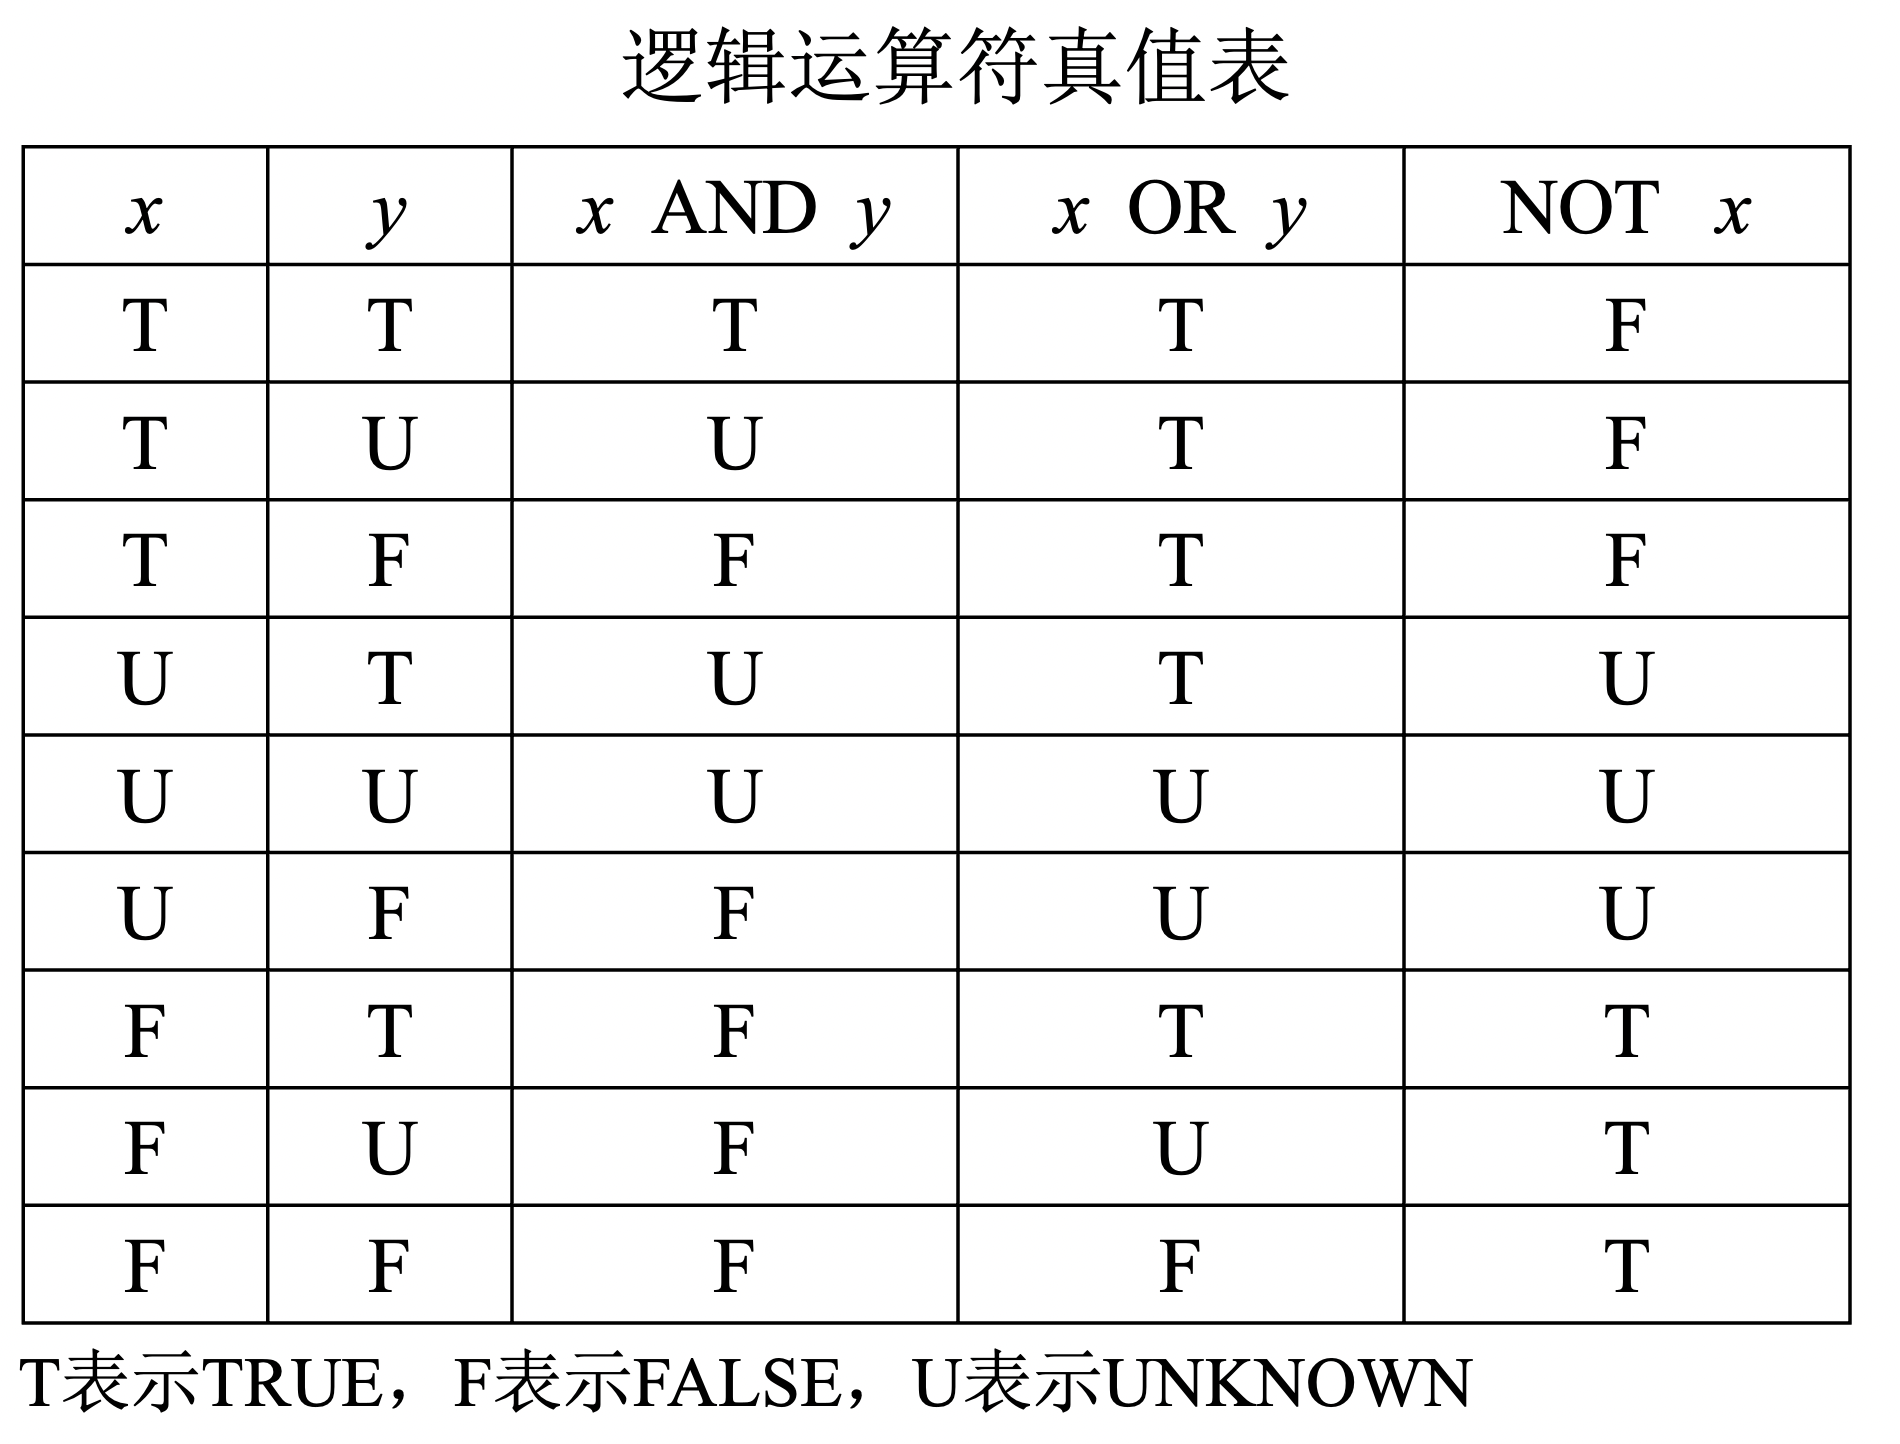
\includegraphics[width=0.5\textwidth]{images/3.5.4}
    \vspace{-1em}
\end{figure}

在查询语句中,只有使\sverb|WHERE|\ 和 \sverb|HAVING|\ 子句的选择条件为TRUE的元组才被选出作为输出结果

例:选出选修1号课程的不及格的学生以及缺考的学生
\begin{lstlisting}
SELECT Sno
FROM SC
WHERE Cno = '1' AND (Grade < 60 OR Grade IS NULL);
\end{lstlisting}
或者
\begin{lstlisting}
SELECT Sno
FROM SC
WHERE Grade < 60 AND Cno = '1'
UNION
SELECT Sno
FROM SC
WHERE Grade IS NULL AND Cno = '1'
\end{lstlisting}

\section{视图}
\begin{itemize}
    \item 视图是从一个或几个基本表(或视图)导出的虚表
    \item 数据库中只存放视图的定义,而不存放视图对应的数据
    \item 一旦基表中的数据发生变化,从视图中查询出的数据也随之改变
\end{itemize}

\subsection{定义视图}

\subsubsection{建立视图}
SQL 语言用\sverb|CREATE VIEW|\ 命令建立视图,其一般格式为
\begin{lstlisting}
CREATE VIEW <视图名> [(<列名> [,<列名>]…)]
AS <子查询>
[WITH CHECK OPTION];
\end{lstlisting}

\begin{itemize}
    \item 子查询可以是任意的\sverb|SELECT|\ 语句,是否可以含有\sverb|ORDER BY|\ 子句和\sverb|DISTINCT|\ 短语,则取决于具体系统的实现
    \item \verb|WITH CHECK OPTION|\ 表示对视图进行\sverb|UPDATE|,\verb|INSERT|\ 和 \sverb|DELETE|\ 操作时要保证更新、插入或删除的行满足视图定义中的谓词条件(即子查询中的条件表达式)
    \item 组成视图的属性列名或者全部省略或者全部指定
    \item 如果省略了视图的各个属性列名,则隐含该视图由子查询中\sverb|SELECT|\ 子句目标列中的诸字段组成
    \item 下列情况必须指定组成视图的所有列名
    \begin{itemize}
        \item 某个目标列是聚集函数或列表达式
        \item 多表连接时选出了几个同名列作为视图的字段
        \item 需要在视图中为某个列启用新的更合适的名字
    \end{itemize}
\end{itemize}

例:建立信息系学生的视图,并要求进行修改和插入操作时仍需保证该视图只有信息系的学生
\begin{lstlisting}
CREATE VIEW IS_Student
AS 
SELECT Sno, Sname, Sage
FROM  Student
WHERE  Sdept = 'IS'
WITH CHECK OPTION;
\end{lstlisting}

\subsubsection{删除视图}
\begin{lstlisting}
DROP VIEW <视图名>[CASCADE];
\end{lstlisting}
\begin{itemize}
    \item 该语句从数据字典中删除指定的视图定义
    \item 如果该视图上还导出了其他视图,使用\sverb|CASCADE|\ 级联删除语句,把该视图和由它导出的所有视图一起删除 
    \item 删除基表时,由该基表导出的所有视图定义都必须显式地使用\sverb|DROP VIEW|\ 语句删除 
\end{itemize}

\subsection{查询视图}
关系数据库管理系统执行对视图的查询时,首先进行有效性检查,检查查询中涉及的表、视图等是否存在。如果存在,则从数据字典中取出视图的定义,把定义中的子查询和用户的查询结合起来,转换成等价的对基本表的查询,然后在执行修正了的查询。这一转换过程称为\textbf{视图消解}。

例:查询选修了1号课程的信息系学生
\begin{lstlisting}
SELECT IS_Student.Sno,Sname
FROM IS_Student,SC
WHERE IS_Student.Sno = SC.Sno AND SC.Cno = '1';
\end{lstlisting}

\subsection{更新视图}
\begin{itemize}
    \item 由于视图是不实际存储数据的虚表,因此对视图的更新最终要转换成对基本表的更新
    \item 像查询视图一样,对视图的更新操作也是通过视图消解,转换为对基本表的更新操作
    \item 一般地,行列子集视图是可更新的
    \item 对其他类型视图的更新不同系统有不同限制。一些视图是不可更新的,因为对这些视图的更新不能唯一地有意义地转换成对相应基本表的更新
\end{itemize}

例:将信息系学生视图\sverb|IS_Student|\ 中学号“201215122”的学生姓名改为”刘辰”
\begin{lstlisting}
UPDATE IS_Student
SET Sname= '刘辰'
WHERE Sno = '201215122';
\end{lstlisting}

转换后的更新语句为:
\begin{lstlisting}
UPDATE Student
SET Sname = '刘辰'
WHERE Sno = '201215122' AND Sdept = 'IS';
\end{lstlisting}

\subsection{视图的作用}
\begin{itemize}
    \item 视图能够简化用户的操作
    \item 视图使用户能以多种角度看待同一数据,适应数据库共享的需要
    \item 视图对重构数据库提供了一定程度的逻辑独立性
    \item 视图能够对机密数据提供安全保护
    \item 适当的利用视图可以更清晰的表达查询
\end{itemize}
	
	% \begin{figure}[H]
    % \vspace{-0.5em}
	% \centering
	% \includegraphics[width=0.4\textwidth]{images/}
    % \vspace{-1em}
	% \end{figure}

	% \vspace{-0.5em}
	% \begin{multicols}{2}
    % \begin{itemize}
    %     \item 
    % \end{itemize}
	% \end{multicols}
	% \vspace{-1em}


\end{document}


